\documentclass{article}

\usepackage{amsfonts}

\usepackage{graphicx}
\graphicspath{ {./images/} }

\usepackage{bm}



\usepackage{amsmath}

\usepackage[a4paper, total={6in, 8in}]{geometry}


\setlength{\parindent}{0pt} % for getting rid of first line indentation


% ================================================
% =====================  BEGIN DOCUMENT 
% ================================================

\title{Game Theory Project}
\author{Juan Pablo Bello Gonzalez}
\date{September 2024}

\begin{document}


\maketitle

\section{introduction}

extensive form games to model imperfect information games. They involve sequential decisions when players choose actions at differnt times (Prof Bryce Extensive Games).
To represent these interactions we can use the extensive form gametree which lets us encode the timing information of a sequential game

"the key idea is tht if player are making decisions at different times, then each point where a player makes a decision is represented as a node in a tree. We'll label the node with the player who is making the decision at that point. Also each level on the tree alternates players. And decisions avaliable to a player when they are making a decision will result in branches steming from that node. Those branches may lead to other decision nodes for various players in the game or they may lead to a terminal outcome represented by a leaf in the tree where as usual we will have a payoff for each of the players, in the case of poker and Khun poker this payoff will be zero sum. "

these levels of the tree correspond to a player making a decision and then player 2 reacting to that decision. This is a computationally intensive method (do poker tree start) even after symmetries removed. 

How strategies and equillibria relate to this model?
- We think of a strategy in an extensive form game as a complete contingent plan of actin that a player would do at any of their decision nodes, given the history wich is visible to them. 
So a strategy for player i takes as input any of the decision nodes for that player and produces an action that the player would play at that possition. 


Counter factual regret minimization. 

How this can be used to model poker and weakly solve poker 


\subsubsection{Modeling imperfect information}

"To model imperfect information, the histories of each player $d$ are partitioned into a collection $d$
of so-called information sets. Each information set $d$
 groups together histories that Player i cannot
distinguish between when he or she acts  (MIT LECTUREs)" For instance, in the case of Kuhn poker, An information set of player 1 is ${JQ, JK}$ which occurs after the draw and before any betting, at this point in time, Player 1 only has knowelde of what eh drew, J in this case. But his information set is bigger since, from his poov, P1 cannot know if P2 has Q or K. 

%%% Define Kuhn poker and DRAW THE Kuhn poker tree here %%%




\section{Formulating an extensive-form game}
According to (REGRET MINIMIZATION..)
A formal definition of an extensive game includes the following:


\begin{itemize}
\item A finite \textbf{set of players} $N$
\item A finite set of ordered action \textbf{histories} $H$, such that the empty sequence is in H and every prefix of a sequence in H is also in H. 
\begin{itemize}
\item Denote $Z \subseteq H$ as the set of terminal histories, corresponding to the leaves of the tree representation, where the game ends, it is no one's turn, and players receive their utilities.
\item Denote $A(h) = \{ a : (h,a) \in H \setminus Z\}$ as the actions available for the player whose turn it is after a non-terminal history $h \ in H \setminus Z$.
\end{itemize}

\item A \textbf{player function}, $P: H \setminus Z \rightarrow N$ that specifies the player whose turn it is to act at the end of a given history.

\item A function $f_i$ that assigns, to every history $h$ where it is player $i$'s turn ($P(h) = i$), a probability measure over the possible actions $A(h)$ at that history. Specifically, $f_i(a|h)$ denotes the probability of player $i$ choosing action $a$ given $h$, with each such probability measure being independent of all others.


\item For each player $i \in N$ define their \textbf{information partition}, $\mathcal{I}_i$, as a partition of the set of histories where player $i$ is required to act, $\{ h \in H : P(h) = i \}$. Each member of the partition $I_i \ in \mathcal{I}_i$ is called an information set and it 
represents the subset of histories indistinguishable to player $i$, based on the information available to them at a specific point in time.

Information sets have the property that for all $h, h' \in I_i$, the available actions must be the same, i.e., $A(h) = A(h')$. 
\item For each player $i \in N$ define a utility function $u_i: Z \rightarrow \mathbb{R}$ that assigns a real-valued utility to each terminal state $z \in Z$. In extensive form games, player actions may occur at various points in time throughout the game, but utilities are assigned exclusively at the terminal states.

\end{itemize}


\section{Formulating Kuhn Poker as an extensive form game}

%%% IMAGE
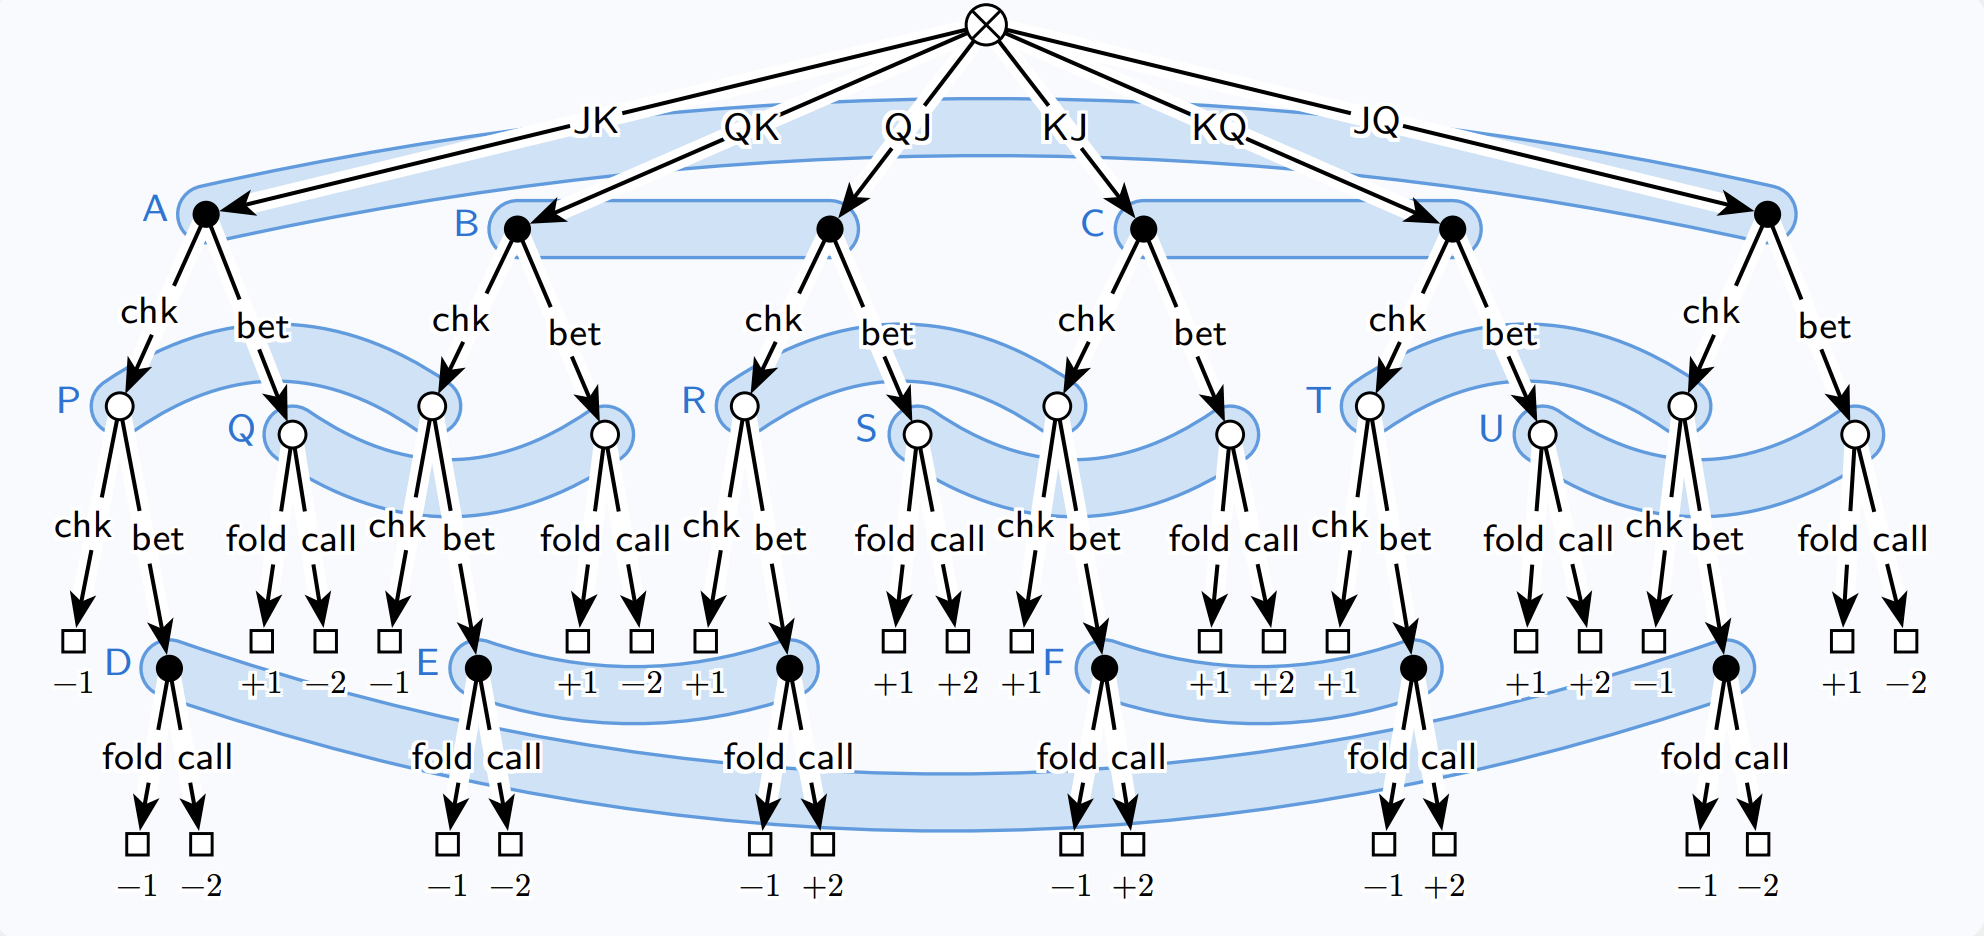
\includegraphics[scale=.44]{game_tree}


In the case of Kuhn poker, there are two players $N = \{1,2 \}$. 


To define the set of histories $H$, one can conceptualize the game as evolving through levels of a decision tree:

\begin{itemize}
\item Level 0 (Root Node):
\begin{itemize}
\item At time 0, nature deals one card to each player from the set $\{J, Q, K \}$.
\item The set of possible cards dealt is $\text{CARDS}  = \{ (c_1, c_2) : c_1, c_2 \in \{J, Q, K \}, c_1 \neq c_2 \}$.
\end{itemize}
\item Level 1:
\begin{itemize}
\item Player 1, knowing their card but not Player 2's, takes an action.
\item The actions available to Player 1 are $A_1 = \{\text{CHECK}, \text{BET}\}$.
\end{itemize}
\item Level 2:
\begin{itemize}
\item Player 2 responds to Player 1's action. 
\item The actions available depend on Player 1's choice:
If Player 1 CHECKS, Player 2 can choose: $\{ \text{CHECK}, \text{BET} \}$. If Player 1 BETS, Player 2 can choose $\{ \text{FOLD}, \text{CALL} \}$. So, in general, Player 2's first action at level 2 is from the union of these two sets, $A_2 = \{\text{CHECK}, \text{BET}, \text{FOLD}, \text{CALL} \}$ 
\end{itemize}
\item  Level 3: 
\begin{itemize}
\item If the game continues (i.e., Player 2 bet as a response to Player 1 checking first), Player 1 has the final decision: $A_3 = \text{FOLD}, \text{CALL}$.
\end{itemize}
\end{itemize}

So, $H$ has the form: 

\[ H \subseteq \text{CARDS} \times A_1 \times A_2 \times A_3 \]

Some example histories are: 
\begin{itemize}
\item Q.K.BET.FOLD
\item K.J.BET.CALL
\item K.J.CHECK.BET.CALL
\end{itemize}

Note that the histories alternate players, so $P(h)= 1$ for histories $h$ of even length such as $Q.K$ and $Q.K.CHECK.BET$. Similarly, $P(h) = 2$ for histories of odd length such as $Q.K.BET$.

Histories also show complete information. Players themselves are not able to see histories, only their respective information sets. 

Each player has 6 information sets. 
Player 1 has three at Level 1 and 3 at level 3. 
Player 2 has 6 at level 2, the only level at which he is allowed to make a move. 


\subsubsection{A strategy in an extensive form game}
'Loosely speaking, a strategy describes how to act in every single possible situation. It is a recipe for how to act in entire game, a lookup table you can read your actions from. (INT8)'

For player i, a strategy should provide a probability distribution over actions available to him at every information set where he is expected to perform an action, so not including terminal nodes. For khun poker: 

%%% LITTLE TABLES. 

\subsubsection{Information sets}
For definining imperfect information sets, players do not have knoweldge of the entire state, player's perspectives are called information sets. 
"Information set is a set of game states (game tree nodes) that are not distinguishable for a player."



\subsubsection{Nash Equilibrium}
By Nash's Theorem, any finite game is guaratneed to have a, possibly mixed, NE. This includes poker and Khun poker. 


\subsubsection{No Regret Learning}

Regret is a key concept in \textit{online learning}, where decisions are repeatedly made in imperfect information environments. Imagine receiving predictions from \( N \) experts for a single phenomenon evolving in discrete time (e.g. a stock price). The sequential nature of such phenomenons like a stock price, means that we can have a prediction

for the price at time t and then observe the actual value of the stock at time t. 

At each time step \( t \), an online algorithm \( \mathcal{A} \) assigns trust to these experts by proposing a probability distribution vector \( p_t \) over them. In the stock example, we may assign a probability distribution for the one step increments over the integers. 
Then, the environment reveals the true outcome, resulting in a loss vector \( l_t \), where each entry represents the loss for an expert's advice. The algorithm's expected loss at time $t$ can then be computed.

We can also compute the total expected loss of $\mathcal{A}$ until time $T$, and the total loss for a single expert util time $T$.

"Regret at time T is then a difference between our algorithm total loss and the best single expert loss... It indeed expresses how much we regret not following the single best expert advice in all time steps.

\textbf{In the context of games, regret will represent the utility we gave up by choosing actions other than the best response.}   

No-regret learning occurs when an online algorithm \( \mathcal{A} \) ensures that, as the number of rounds \( T \) approaches infinity, its average regret approaches zero, even in the worst-case scenario. This means \( H \) performs at least as well as any single expert in the long run, with no regret toward any individual expert.

\subsubsection{Regret matching as an example of no-regret learning algorithm}
EXPERTS are actions (ie you shuold fold, call, bet)

The Regret Matching algorithm \( \hat{H} \) maintains a vector of weights assigned to experts. After the loss vector (representing the consequences of the experts' advice) is revealed, the cumulative regret for each expert \( i \) at time \( t \) is computed. This cumulative regret indicates how much the algorithm regrets not following a particular expert \( i \)'s advice.

\[ R_{i,t} = L^t_{\mathcal{A}} - L^t_i \]

And after each iteration, expert weights can be updated with the formula: 
\[ w_{i,t} = \max(0, R_{i,t}) \]

And finally update the vector....

\subsubsection{No-regret learning and game theory}
%% This section is iffy, may not even be accurate.
Relate no regret learning to game theory. 
 
This regret matching algorithm can be used to model something that evolves with time, but the issue with games is that we would like to input the game state/history at some point into the regret,

Since regret goes from costs to utility, we now wish to maximize it?

Both players in fact will adapt to one another via no-regret learning. So how do we keep track of the regret for each plater?

\textbf{THEOREM:}
If two no-regret algorithms play a zero-sum game against one another for T iterations with average regret less than $\epsilon$, then their average strategies approximate Nash Equilibrium (up to $2 \epsilon$) 

\subsubsection{Regret Minimization}
Average overall regret for player $i$ at time $T$ is defined as:
\[ R^T_i = \max_{\sigma^*_i \in \Sigma_i} \sum_{t=1}^T (u_i(\sigma^*_i, \sigma_{-i}^t) - u_i(\sigma^t)) \]

It expresses how much we regret not playing single fixed best response to all strategies our opponent played up until T. 

Also consider the average strategy for player $i$ from time 1 to $T$

\[ \bar\sigma^t_i (I)(a) = \frac
{\sum_{t=1}^T \pi_i^{\sigma^t}(I) \times  \sigma^t (I)(a)} 
{\sum_{t=1}^T \pi_i^{\sigma^t}(I)} \]

THEOREM: In a two-player zero-sum game at time T, if both player's average overall regret is less than $\epsilon$, then $\bar\sigma^T$ is a $2 \epsilon$ equilibrium

This means that if both players aim to minimize average overall regret, their average strategies will converge to an approximation Nash Equilibrium as $T \to \infty$. Ans so a corollary of this result is that a regret minimizing algorithm is capable of computing an approximate Nash equillibrium. 

We cannot immediatly proceed with Regret minimization because, to compute regret we need knowedlge each player's best response $\sigma^*_i \in \Sigma_i$. If we knew those straategies, it would be trivial to construct a Nash equilllibrium. 

Instead of computing overall regret, the aproach is to decompose overall regret into a set of additive, 'made up' regerts based on the information sets avalaible to player i, that can be minimized independently. These are called counterfactual regrets. 

""
First consider one particular information set $I \in \mathcal{I}_i$ and player $i$’s choices made in that
information set.

Define counter-factual utility $u_i( \sigma, I)$ to be the expected utility given that information set I is reached and all players play using strategy $\sigma$  except for player $i$, who plays to reach that information set $I$. 

Formally if $\pi ^{\sigma}(h, h')$ is the probability of going from history $h$ to terminal history $h'$, then the counterfactual utility at information set $I$ is given by:

\[ u_i(\sigma, I) = \frac{sum_{h \in I, h' \in Z} \pi_{-i}^{\sigma}(h) \pi^{\sigma}(h, h')u_i(h')}{\pi_{-i}^{\sigma}(I)} \]

With this counterfactual utility, we can now define immediate counterfactual regret. for all $a \in A(I)$, let $\sigma|_{I \rightarrow a}$ denote the strategy profile identical to $\sigma$ except that player $i$ always chooses action $a$ when in information set $I$. This will enable us to write the immediate conunterfactual regret: 
\[
R_{i, imm}^T(I) = \frac{1}{T} \max_{a \in A(i)} \sum_{t=1}^T \pi_{-i}^{\sigma^t}(I)(u_i(\sigma^t|_{I \rightarrow a}, I) - u_i(\sigma^t, I)) 
\]

This conterfactual  regret is in terms of the best responses  at information set $I$, whereas regular average regret is in terms of all possible strategic profiles $\Sigma_i$, making it much more manageable as information sets are finite with a finite set of possible actions. 

This measures the regret a player feels about their decisions limited to the information set $I$, based on the counterfactual utility which in turn is the regret from not choosing the best response at the information set $I$. finding best responses for individual information sets is much simpler than trying to find best responses for the entire game at once, that is the key step in counterfactual regrets. 

It includes a weighting factor that accounts for how likely $I$ would have been reached if the player had actively tried to reach it during that round. Since we are often most concerned with regret only when it is positive, we define the positive part of immediate counterfactual regret as:

\[ R_{i,imm}^{T,+} = \max(0, R_{i,imm}^T(I)) \]


It is clear that minimizing counterfactual regrets at every information set is a much simpler task than minimizing regret over the whole strategy profile $\sigma_i$ all at once, however, so far we only have a result from the the theory of no-regret learning that minimizing regret produces an approximation Nash equillibrium, so we would like a result that says that we can minimize the sum of immediate counterfactual regrets as a proxy for average regret and still obtain a nash equilibrium when the best responsesn at information sets are aggregated into a full strategy. The result in questions was proved by Zinkevich and is as follows:

\[ R^T_i \leq \sum_{I \in \mathcal{I}_i} R_{i,imm}^{T,+}(I) \]

By this result, minimizing immediate counterfactual regret also minimizes overall regret, as the total regret for player $i$ is bounded by the sum of their immediate counterfactual regrets.


\subsection{Results}
Modifying a regret



\end{document}
